\documentclass[a4paper,11pt]{article}

\usepackage[utf8]{inputenc}
\usepackage[czech]{babel}
\usepackage[left=2cm,top=3cm,text={17cm,24cm}]{geometry}
\usepackage{graphicx}
\usepackage{listings}
\usepackage{url}

\title{Systém DNS\\
{\bf\large ISA - Laboratorní cvičení č.3}\\
{\bf\large Prokotol ke cvičení}}

\author{Vysoké učení technické v Brně}

\date{\url{https://github.com/nesfit/ISA/tree/master/lab3-dns}}

\setlength\parindent{0pt}

\begin{document}

{\let\newpage\relax\maketitle}

Jméno a příjmení:\\
Login:\\
Skupina (číslo nebo čas):\\
Datum:

\section{Služba DNS}
\textbf{1.2} IPv4 adresa serveru {\tt www.vutbr.cz}: \underline{\hspace{8cm}}\\


\textbf{1.3} Podle čeho se pozná, ke kterému dotazu DNS patří daná odpověď? \underline{\hspace{25mm}}\\

\textbf{1.6} Jaký typ záznamů obsahuje autoritativní servery? \underline{\hspace{25mm}}\\

Autoritativní servery DNS pro doménu \texttt{vutbr.cz}:

\vskip 4em

\textbf{1.9} Zjištění typ dotazu DNS? \underline{\hspace{4cm}}\\

\textbf{1.10} Cílová IP adresa paketu dotazu DNS: \underline{\hspace{4cm}}\\

Jak zjistí klient DNS, na který server DNS má posílat dotazy? \underline{\hspace{40mm}}\\

\textbf{1.12.} Primární e-mailový server pro doménu \texttt{fit.vutbr.cz}: \underline{\hspace{45mm}}

\section{Služba Whois}
\textbf{2.1} Ve kterém roce byla registrována doména {\tt vutbr.cz}? \underline{\hspace{3cm}}\\

\textbf{2.2} Nakonfigurovaná IPv4 adresa na rozhraní \texttt{enp2s0}: \underline{\hspace{3.8cm}}\\

Zjištěná veřejná IPv4 adresa: \underline{\hspace{3.8cm}}\\

Proč se veřejná adresa neshoduje s žádnou adresou nakonfigurovanou na vašem počítači?\\

\vskip 2em

\textbf{2.3} Do jakého rozsahu patří Vaše veřejná IP adresa? \underline{\hspace{3.8cm}} -- \underline{\hspace{3.8cm}}\\

Komu je tento  rozsah přidělen?\hspace*{0.2cm}\underline{\hspace{3.8cm}}

\section{Konfigurace vlastního serveru DNS}
\textbf{3.14} Výstup příkazu \texttt{nslookup 10.10.10.1}:
\\
\\
\\
\hspace*{0.7cm} Výstup příkazu \texttt{dig PCUC.xlogin00.cz}:
\\
\\
{\footnotesize \hspace*{0.8cm}ANSWER SECTION:
\\
\\
\\
\hspace*{0.8cm}AUTHORITY SECTION:
\\
\\
\\
\hspace*{0.8cm}ADDITIONAL SECTION:}
\\
\\
\\
\hspace*{0.7cm} Výstup příkazu \texttt{dig -x 10.10.10.1xx}, kde xx je číslo vašeho počítače:
\\
\\
{\footnotesize \hspace*{0.8cm}ANSWER SECTION:
\\
\\
\\
\hspace*{0.8cm}AUTHORITY SECTION:
\\
\\
\\
\hspace*{0.8cm}ADDITIONAL SECTION:}
\\
\\
\\
\textbf{3.19} Doplňte diagram popisující posloupnost dotazů DNS zachycených na rozhraních \texttt{loopback} a \texttt{enp2s0}. Do diagramu napište IP adresy serverů DNS, na které dotaz směroval. Uveďte typy dotazů. 
\\
\\
\hspace*{0.8cm}Zadaný příkaz: \texttt{dig }\underline{\hspace{4.5cm}}
\begin{figure}[h]
	\centering
	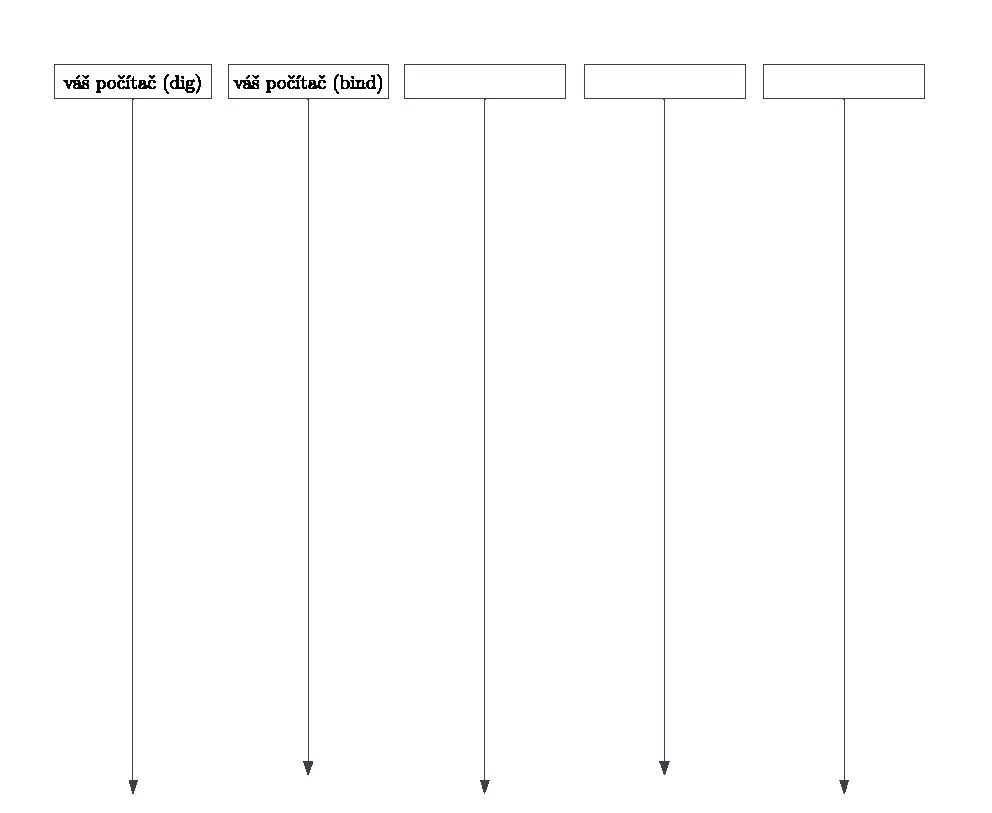
\includegraphics[bb=0 365 550 130, clip=true]{dia.eps}
\end{figure}
\end{document}
